Organize this section according to the rules defined in the project description. 
\subsection{External Interface Requirements}



\subsubsection{User Interfaces}
\subsubsection{App Mockups}

\subsubsection{Hardware Interfaces}
\begin{flushleft}
All users will access the application with their own devices: mobile device, tablet device, or computer device. 
The farmer's device needs the following in order to have full functionality of DREAM:
\begin{itemize}
\item Internet connection [required]: when the farmer is submitting their data while in their fields, their device will need to have an internet connection in order to access DREAM servers.
\item Camera [optional]: farmers can submit pictures to aid their textual descriptions when posting in the discussion board or when messaging their agronomist/s. Although this is not required to use the application, it is highly recommended. 
\item GPS sensor [optional]: farmers can either enter the location for their fields manually or by allowing the application to utilize the GPS sensor from the device. 
\end{itemize}

The agronomist's device needs the following in order to have full functionality of DREAM:
\begin{itemize}
\item Internet connection [required]: when the agronomist is visiting farmers their device will need to have internet access in order for the agronomist to submit their reports to the DREAM servers throughout the day and to follow the navigation path calculated by DREAM.
\item GPS [optional]: since the agronomist will use a navigation plan generated by DREAM, sharing their GPS location is preferred for an optimal user experience. Without this device functionality, the agronomist will not be able to receive turn-by-turn live directions. 
\end{itemize}

The policy maker's device needs the following in order to have full functionality of DREAM:
\begin{itemize}
\item Internet connection [required]: in order to access the rankings and evaluations of the farmers throughout the region, internet connection is required to access the DREAM servers. 
\end{itemize}
\end{flushleft}

\subsubsection{Software Interfaces}
This product is accessible through a mobile-friendly application. Farmers will spend the majority of their time accessing the application through a mobile device; agronomists will access the application with both a mobile device and a computer device; policy makers will access the application almost exclusively with a computer device. Due to the mix of mobile and computer devices, the web application must be suitable for both interfaces. 


\subsubsection{Communication Interfaces}
The mobile-friendly web application will communicate with DREAM servers over an internet connection. 

\subsection{Functional Requirements}
Definition of use case diagrams, use cases and associated sequence/activity diagrams, and mapping on requirements

%Use this counter for the scenarios and command \addOne to print and increase at the same time
\newcounter{usecase_counter}
\setcounter{usecase_counter}{1}

%GENERICS USE CASES
% Use Case Table
\begin{center}
\renewcommand{\arraystretch}{1.25}
\begin{tabular}{|l|>{\raggedright\arraybackslash}m{12cm}|}
    \hline
    \textbf{Name} & User Registration\\
    \hline
   	\textbf{Actor} & Farmer, Agronomist, Policy Maker ???\\
    \hline
    \textbf{Entry Conditions} & \\
    \hline
    
    \textbf{Events Flow} & \begin{enumerate}
    			\item The user register on the site using his/her email.
    			\item The user gets an appointment to verify his/her identity.
    			\item The user profile is validated and obtains credentials.
	    		\end{enumerate}
    	\\
    \hline
    \textbf{Exit Conditions} & \begin{itemize}
    	\item The user has credentials of a validated account.
   		\end{itemize} \\
    \hline
\end{tabular}
\end{center}
% Use Case Table

\begin{center}
\begin{tabular}{|l|>{\raggedright\arraybackslash}m{12cm}|}

    \hline
    \textbf{Name} & \textit{User log-in}\\
    \hline
   	\textbf{Actor} & \textit{Farmer, Agronomist, Telangana's policy maker}\\
    \hline
    \textbf{Entry Conditions} & \textit{The user opens the application}\\
    \hline
    \textbf{Events Flow} & \textit{
    \begin{enumerate}
            \item The user press the "log-in" option on the screen
            \item The user inserts his credentials
            \item The user press the "log-in" button
            \item The user can then choose multiple farmers to visit that day from a list of recommended 					ones
     \end{enumerate}}\\
    \hline
    \textbf{Exit Conditions} & \textit{The system accepts the credentials  and the user is now able to perform actions inside the application}\\
    \hline
    \textbf{Exceptions} & \textit{
      \begin{itemize}
          \item The credentials are not valid, therefore the user will be asked to check her/his input
		\item The password is not correct so the user will be asked to insert the correct password. After three tries, the account is temporarily blocked and a reset mail is sent
        \end{itemize}
     }\\
    \hline
\end{tabular}
\end{center}
%FARMERS
\subsubsection{Farmer}
% Scenario Text
\begin{flushleft}
\textbf{Scenario \addOne{usecase_counter}:} 
Max is a farmer who cultivates some fields near his house in Telangana state. Max has been planting the same plant species over the last few years; he refrains from trying different plants because he is unfamiliar with the cultivation methods. Now, with more children and grandchildren to feed, he would like to change the crop with something more productive. Max learned about the DREAM initiative from a friend and, through the Association of Farmers, he received his credentials to log into the website.
Within minutes of accessing the site, he skimmed through the discussion forums and discovered that there are thousands of small farmers like him with the same doubts and fears. He learned which species are more productive and which fertilizer to use. Now he can feed his entire family and even sell some food to the local market.
\end{flushleft}
% Use Case Table
\begin{center}
\begin{tabular}{|l|>{\raggedright\arraybackslash}m{12cm}|}

    \hline
    \textbf{Name} & \textit{Create a thread in farmers' forum}\\
    \hline
   	\textbf{Actor} & \textit{Farmer}\\
    \hline
    \textbf{Entry Conditions} & \textit{The user uses valid credentials to log into the application}\\
    \hline
    \textbf{Events Flow} & \textit{
    		\begin{enumerate}
    			\item The user opens the forums section
    			\item The user clicks on "Create thread"
    			\item The user writes a valid title and message
    			\item The user clicks on "Publish"
    			\item The user can answer to messages published in his conversation
    		\end{enumerate}
    	}\\
    \hline
    \textbf{Exit Conditions} & \textit{The user closes the forum section or the entire application}\\
    \hline
    \textbf{Exceptions} & \textit{
    		\begin{itemize}
    			\item The server is not available
    		\end{itemize}
    	}\\
    \hline
\end{tabular}
\end{center}
% Use Case Table
\begin{center}
\renewcommand{\arraystretch}{1.25}
\begin{tabular}{|l|>{\raggedright\arraybackslash}m{12cm}|}

    \hline
    \textbf{Name} & Visit the discussion forum\\
    \hline
   	\textbf{Actor} & Farmer\\
    \hline
    \textbf{Entry Conditions} & The logs into the application with valid credentials.\\
    \hline
    \textbf{Events Flow} & 
    		\begin{enumerate}
    			\item The user opens the "Forums" section.
    			\item The user opens a thread and reads the conversation.
    			\item The user submits a post in an existing thread.
    		\end{enumerate}
    	\\
    \hline
    \textbf{Exit Conditions} & \begin{itemize}
    	\item The user exits the "Forum" section.
    	\item The user closes the entire application.\end{itemize}\\
    \hline
    \textbf{Exceptions} & 
    		\begin{itemize}
    			\item The server is not available.
    			\item There are no existing threads.
    		\end{itemize}
    	\\
    \hline
\end{tabular}
\end{center}
% Scenario Text
\begin{flushleft}
\textbf{Scenario \addOne{usecase_counter}:} 
Caroline has a big farm in Telangana state with 50 hectares of land and different varieties of plants. Last year, during the monsoon season, her fields were flooded, and almost no plants survived. In addition, this summer, the hot temperature killed some other species.
After consulting an expert, she decided to join the DREAM initiative to ask for direct support from agronomists and to obtain some incentives from the central government.
Next year she will plant more resilient crops and take some precautions against flooding.
\end{flushleft}
% Use Case Table
\begin{center}
\begin{tabular}{|l|>{\raggedright\arraybackslash}m{12cm}|}

    \hline
    \textbf{Name} & \textit{Asking advice to agronomists}\\
    \hline
   	\textbf{Actor} & \textit{Farmer}\\
    \hline
    \textbf{Entry Conditions} & \textit{The user uses valid credentials to log into the application}\\
    \hline
    
    \textbf{Events Flow} & \textit{
    		\begin{enumerate}
    			\item The user opens the "Ask to experts" section
    			\item The user selects the assigned agronomist
    			\item The user writes a short request and submit it
    			\item After receiving a notification, The user can see the answer
    			\item Eventually, The user can continue the conversation asking further questions
    		\end{enumerate}
    	}\\
    \hline
    \textbf{Exit Conditions} & \textit{The conversation is closed by either the farmer or the agronomist}\\
    \hline
    \textbf{Exceptions} & \textit{
    		\begin{itemize}
    		    	\item The server is not available
    			\item The agronomist doesn't answer to the message
    		\end{itemize}
    }\\
    \hline
\end{tabular}
\end{center}
% Use Case Table
\begin{table}[hbt!]
\centering
\caption{\label{table:addOne{table_counter}}Farmer use case.}
\renewcommand{\arraystretch}{1.25}
\begin{tabular}{|l|>{\raggedright\arraybackslash}m{12cm}|}

    \hline
    \textbf{Name} & Add field location with GPS\\
    \hline
   	\textbf{Actor} & Farmer\\
    \hline
    \textbf{Entry Conditions} & The user logs into the application with valid credentials and is physically in the field.\\
    \hline
    \textbf{Events Flow} & 
    		\begin{enumerate}
    			\item The user opens the "My Farm" section.
    			\item The user clicks on the "Add New Field" button.
    			\item The user is prompted to allow the application to use their GPS location.
    			\item The user clicks on the "Allow" button, allowing the application to locate them using GPS.
    			\item The user adds information about the size of the field, crop currently planted, the fertilizer in use, and any other information they deem relevant.
    			\item The user clicks on the "Submit" button.
    		\end{enumerate}
    	\\
    \hline
    \textbf{Exit Conditions} & The user submits the information about the new field.\\
    \hline
    \textbf{Exceptions} & 
    		\begin{itemize}
    			\item The server is not available.
    			\item The application is not able to use the GPS.
    			\item The user doesn't allow the application to use GPS.
    			\item The provided information is not valid.
    			\item Some required information is left empty.
    		\end{itemize}
    \\
    \hline
\end{tabular}
\end{table}
% Use Case Table
\begin{table}[hbt!]
\centering
\caption{\label{tab:addOne{table_counter}}Farmer use case related to Scenario 2.}
\renewcommand{\arraystretch}{1.25}
\begin{tabular}{|l|>{\raggedright\arraybackslash}m{12cm}|}

    \hline
    \textbf{Name} & Upload information about production\\
    \hline
   	\textbf{Actor} & Farmer\\
    \hline
    \textbf{Entry Conditions} & The user logs into the application with valid credentials and has new data to upload.\\
    \hline
    
    \textbf{Events Flow} & 
    		\begin{enumerate}
    			\item The user opens the "My Production" section.
    			\item The user clicks on the "Update Production Data" button.
    			\item The user selects a field to update from a list of fields.
    			\item The user adds the desired information.
    			\item The user clicks on the "Submit" button.
    		\end{enumerate}
    	\\
    \hline
    \textbf{Exit Conditions} & The user submits the information.\\
    \hline
    \textbf{Exceptions} & 
    		\begin{itemize}
    			\item The server is not available.
    			\item The provided information is not valid.
    			\item Some required information is left empty.
    		\end{itemize}
    \\
    \hline
\end{tabular}
\end{table}
% Use Case Table
\begin{center}
\renewcommand{\arraystretch}{1.25}
\begin{tabular}{|l|>{\raggedright\arraybackslash}m{12cm}|}
    \hline
    \textbf{Name} & Access weather forecast data\\
    \hline
   	\textbf{Actor} & Farmer\\
    \hline
    \textbf{Entry Conditions} & The user logs into the application with valid credentials and has at least one field registered with the application.\\
    \hline
    
    \textbf{Events Flow} & \begin{enumerate}
    			\item The user opens the "My Farm" section.
    			\item The user clicks on the "Weather" tab.
    			\item The user selects a field from a list of fields.
    			\item The user can see the weather associated with the location for the selected field.
	    		\end{enumerate}
    	\\
    \hline
    \textbf{Exit Conditions} & \begin{itemize}
    	\item The user closes the weather section.
    	\item The user navigates "Back" to the list of fields.
   		\item The user closes the entire application.
   		\end{itemize} \\
    \hline
    \textbf{Exceptions} &
    		\begin{itemize}
    			\item The server is not available.
    		\end{itemize}
    \\
    \hline
\end{tabular}
\end{center}

%AGRONOMISTS
\subsubsection{Agronomist}
%before: emails for help, data, now can consult
% Scenario Text
\begin{flushleft}
\textbf{Scenario \addOne{usecase_counter}:} 
Schmidt is an agronomist. His job is based on knowing farmers' information and helping them to improve and solve problems. Before installing DREAM he was receiving various emails from farmers. All the emails contained important information about them and help or suggestion requests. He then needed to combine the content from the emails with the information he provided about latest visits of their farm. Sometimes data were not in the same format and not standardized; this slowed his work. Now with DREAM he can easily inspect all of the data in the same place from the convenience of his device. Data are more readable and available. He can also now consult them in any place with an internet connection.
\end{flushleft}

%respond to help req
% Use Case Table

\begin{table}[hbt!]
\centering
\small
\caption{\label{tab:agrRespondHelp}Agronomist responding to help requests from farmers in their subarea..}
\renewcommand{\arraystretch}{1.25}
\begin{tabular}{|l|>{\raggedright\arraybackslash}m{12cm}|}

    \hline
    \textbf{Name} & Respond to help requests\\
    \hline
   	\textbf{Actor} & Agronomist\\
    \hline
    \textbf{Entry Conditions} & The user has opened the application, logged in with valid credentials, specified their responsible area, and received at least one help request.\\
    \hline
    \textbf{Events Flow} & \begin{enumerate}
            \item The user clicks on the "Help Requests" button.
            \item The user views the list of the the different help requests received from different farmers.
            \item The user can select a farmer from the list of help request and inspect data about the farmer such as location, ranking, and evaluation.
            \item The user reads the help requests and can then reply with solutions and suggestions.
       \end{enumerate}\\
    \hline
    \textbf{Exit Conditions} & \begin{itemize}
    	\item The user has answered to the farmer and the response has been sent to the farmer.
    	\item The user navigates out of the "Help Requests" section.
    \end{itemize}\\
    \hline
    \textbf{Exceptions} & 
       \begin{itemize}
          \item The messages are not accessible at the moment the user is asked to try again later.
          \item A message cannot be sent in this moment the user is asked to try again later.
        \end{itemize}
     \\
    \hline
\end{tabular}
\end{table}

%visits, daily plan, info on performance, suggests path, confirm plan
% Scenario Text
\begin{flushleft}
\textbf{Scenario \addOne{usecase_counter}:} 
Cece is an agronomist. Part of her job is to visit farms in the area. She has to establish a daily plan for her visits and then send all the data she collects to the Telangana authorities. The daily plan his very hard to create, she has to search for farmers that need more help then others and find a path that connects all their farms. She also has to keep an eye on distance between farms and how to reach them. She installs DREAM and now her work is much easier. All of the info about farmers location, performance and needs are in one place. The system also recommends farmers to visit and automatically suggest a path connecting all the farms. At the end of a day of visits she has to compile the form about farmers performance that are sent automatically to the Telangana authorities.
\end{flushleft}

%create daily plan
% Use Case Table

\begin{center}
\begin{tabular}{|l|>{\raggedright\arraybackslash}m{12cm}|}

    \hline
    \textbf{Name} & \textit{Daily plan creation}\\
    \hline
   	\textbf{Actor} & \textit{Agronomist}\\
    \hline
    \textbf{Entry Conditions} & \textit{The agronomist has opened the app and is logged in}\\
    \hline
    \textbf{Events Flow} & \textit{\begin{enumerate}
            \item The user clicks on the daily plans interface
            \item The user clicks on create a new daily plan
            \item The user chooses a day from a calendar
            \item The user can then choose multiple farmers to visit that day from a list of recommended ones
            \item Whenever a farmer is added to the daily plan the system recalculates the best path that connects all selected farmers and updates the map
       \end{enumerate}}\\
    \hline
    \textbf{Exit Conditions} & \textit{The daily plan is created and inserted in the “your daily plans” section by the system}\\
    \hline
    \textbf{Exceptions} & \textit{
      \begin{itemize}
          \item 
        \end{itemize}
     }\\
    \hline
\end{tabular}
\end{center}
%confirm daily plan
% Use Case Table

\begin{table}[hbt!]
\centering
\small
\caption{\label{tab:agrConfirmPlan}Agronomist accessing the daily plan interface to confirm a daily plan after visiting farmers.}
\renewcommand{\arraystretch}{1.25}

\begin{tabular}{|l|>{\raggedright\arraybackslash}m{12cm}|}

    \hline
    \textbf{Name} & Confirming a daily plan\\
    \hline
   	\textbf{Actor} & Agronomist\\
    \hline
    \textbf{Entry Conditions} & The user has opened the application, logged in with valid credentials, specified their responsible area, and created a daily plan for that specific day.\\
    \hline
    \textbf{Events Flow} & \begin{enumerate}
            \item The user click on the daily plan interface.
            \item The user clicks on the "Your Daily Plans."
            \item The user can then choose a specific daily plan and view or modify the information.
       \end{enumerate}\\
    \hline
    \textbf{Exit Conditions} & The plans are correctly modified and saved by the system\\
    \hline
    \textbf{Exceptions} & 
       \begin{itemize}
          \item The database with daily plans data is not accessible at the moment the user is asked to try again later.
        \end{itemize}
     \\
    \hline
\end{tabular}
\end{table}

%viewing ranking
% Use Case Table

\begin{table}[hbt!]
\centering
\small
\caption{\label{tab:agrViewRank}Agronomist Use Case: View Rank.}

\begin{tabular}{|l|>{\raggedright\arraybackslash}m{12cm}|}

    \hline
    \textbf{Name} & Viewing the ranking\\
    \hline
   	\textbf{Actor} & Agronomist\\
    \hline
    
    %The user logs into the application with valid credentials
    \textbf{Entry Conditions} & The user has opened the application, logged in with valid credentials, and specified their responsible area. \\
    \hline
    \textbf{Events Flow} & \begin{enumerate}
            \item The user clicks on the farmers ranking interface.
            \item The user can view general statistics of the area.
            \item The user can click on any farmer to view their evaluation and statistics.
       \end{enumerate}\\
    \hline
    \textbf{Exit Conditions} & The user selects another tab to exit the ranking view.\\
    \hline
    \textbf{Exceptions} & 
       \begin{itemize}
          \item The database of farmers performance is not accessible.% at the moment the user is asked to try again later.
        \end{itemize}
     \\
    \hline
\end{tabular}
\end{table}
% sending report
% Use Case Table
\begin{table}[hbt!]
\centering
\caption{\label{tab:addOne{figure_counter}}Use case for Agronomist.}

\renewcommand{\arraystretch}{1.25}
\begin{tabular}{|l|>{\raggedright\arraybackslash}m{12cm}|}
    \hline
    \textbf{Name} & Sending a report\\
    \hline
   	\textbf{Actor} & Agronomist\\
    \hline
    \textbf{Entry Conditions} & The user has opened the application, logged in with valid credentials, and specified their responsible area.\\    
    \hline
    \textbf{Events Flow} & 
    	\begin{enumerate}
            \item The user clicks on the daily plan interface.
            \item The user click on the daily plan of the day and selects a farmer also based on the GPS position.
            \item The user can fill a form about the farmer's data, evaluation and 
       \end{enumerate}\\
    \hline
    \textbf{Exit Conditions} & The user has correctly sent the information to the server and the data have been saved.\\
    \hline
    \textbf{Exceptions} & 
    	\begin{itemize}
	    	\item The server is not accessible at the moment.
    	\end{itemize}\\
    \hline 
\end{tabular}
\end{table}


%choosing location
% Use Case Table

\begin{center}
\begin{tabular}{|l|>{\raggedright\arraybackslash}m{12cm}|}

    \hline
    \textbf{Name} & \textit{Choosing the location}\\
    \hline
   	\textbf{Actor} & \textit{Agronomist}\\
    \hline
    \textbf{Entry Conditions} & \textit{The user has opened the app and is logged in}\\
    \hline
    \textbf{Events Flow} & \textit{\begin{enumerate}
            \item The user open the "My area" section of the application
            \item The user selects the area he/she his responsible of on a map
       \end{enumerate}}\\
    \hline
    \textbf{Exit Conditions} & \textit{The system saves the area chosen }\\
    \hline
    \textbf{Exceptions} & \textit{
        \begin{itemize}
          \item The site is not accessible at the moment so the user is asked to try again later
        \end{itemize}
     }\\
    \hline
\end{tabular}
\end{center}

%inspect weather forecast
% Use Case Table
\begin{table}[hbt!]
\centering
\small
\caption{\label{tab:agrWeather} Agronomist Use Case: Accessing Weather.}
\renewcommand{\arraystretch}{1.25}
\begin{tabular}{|l|>{\raggedright\arraybackslash}m{12cm}|}
    \hline
    \textbf{Name} & Inspecting weather forecasts\\
    \hline
   	\textbf{Actor} & Agronomist\\
    \hline
    \textbf{Entry Conditions} & The user has opened the application, logged in with valid credentials, and specified their responsible area.\\    
    \hline
    \textbf{Events Flow} & 
    	\begin{enumerate}
            \item The user clicks on the weather forecast interface.
            \item The user clicks on a section of their responsible area.
            \item The user inspects the weather forecast for the selected area.
       \end{enumerate}\\
    \hline
    \textbf{Exit Conditions} & The user exits the weather forecast section.\\
    \hline
    \textbf{Exceptions} & 
    	\begin{itemize}
	    	\item The data about weather forecast is not accessible.
    	\end{itemize}\\
    \hline 
\end{tabular}
\end{table}


%POLICY MAKERS
\subsubsection{Policy Maker}
%%%% remove this
\begin{flushleft}
\textbf{Scenario \addOne{usecase_counter}: Configuring Ranking Views and Flagging Farmers}\\\smallskip
Ernie is a policy maker within the Teleagana government tasked with identifying the poor-performing farmers in the region. This year, a popular fertilizer manufacturer called NaturGrow slightly changed their formula. Aware of this, Ernie uses the DREAM system to view the ranking of all the farmers in the region and compare rankings by the type of fertilizer each farmer uses. Ernie observes that farmers using the new formula of NaturGrow observed a greater increase their yields compared to the other farmers. Ernie uses this information to flag the farmers who did not see an increase in their yields and did not use NaturGrow's new formula. 
\end{flushleft}


\begin{flushleft}
\textbf{Scenario \addOne{usecase_counter}: Setting Triggers}\\\smallskip
Winston is a policy maker within the Telangana government tasked with providing a mid-season status report on the progress of the farmers. Winston configures his view to organize the ranking of the farmers by water usage. Winston notices a group of outliers over-consuming water but producing below-average yields. Winston sets a trigger to alert agronomists when farmers in their responsible area surpass the average water usage while yielding below-average production. This trigger classifies such farmers as "poor-performing" in the DREAM system. 
\end{flushleft}

% setting triggers

% Use Case Table
\begin{center}
\begin{tabular}{|l|>{\raggedright\arraybackslash}m{12cm}|}

    \hline
    \textbf{Name} & \textit{Set Trigger}\\
    \hline
   	\textbf{Actor} & Policy Maker\\
    \hline
    \textbf{Entry Conditions} & User is logged in as a policy maker with valid credentials.\\
    \hline
    \textbf{Events Flow} & 
    \begin{enumerate}
	    \item Policy maker clicks on "Create trigger" button.
    	\item Policy maker is navigated to the create trigger wizard.
    	\item Policy maker selects the parameters and limits for the trigger.
    	\item Policy maker clicks on the "submit button"
    \end{enumerate} \\ \hline
    \textbf{Exit Conditions} & Sufficient information is provided to set the trigger and the trigger is entered into the system\\
    \hline
    \textbf{Exceptions} & Limits are missing for the parameters selected.\\
    \hline
\end{tabular}
\end{center}
%flagging poor perf

% Use Case Table
\begin{table}[H]
\centering
\small
\caption{\label{tab:policyUseFlag}Policy Maker Use Case: Flagging Farmers.}
\renewcommand{\arraystretch}{1.25}
\begin{tabular}{|l|>{\raggedright\arraybackslash}m{12cm}|}
    \hline
    \textbf{Name} & Flagging Poor-Performing Farmers\\
    \hline
   	\textbf{Actor} & Policy Maker\\
    \hline
    \textbf{Entry Conditions} & The user has logged in with valid credentials and configured a ranking view.\\
    \hline
    \textbf{Events Flow} & 
    \begin{enumerate}
    	\item The user scrolls the low-ranking section of the list.
    	\item The user clicks on the grey "flag" icon for each respective farmer they would like to flag. 
    \end{enumerate}\\
    \hline
    \textbf{Exit Conditions} & The flag icon turns red.\\
    \hline
    \textbf{Exceptions} & The database is unavailable.\\
    \hline
\end{tabular}
\end{table}

\begin{flushleft}
\textbf{Scenario \addOne{usecase_counter}: DREAM helping drive policy decisions}\\\smallskip
The Telangana government partners with a start-up that is developing a new agriculture tool aimed at reducing the manual labor involved in cultivating castor. Jessica, a Telangana policy maker, rolls out a beta program steered by agronomists to issue this new product to various farmers across the region and observe how the product affects castor crop quality and production yields. Jessica observes that farmers participating in the beta program are generating much greater production yields compared to farmers not in the beta program. The increased production yields qualifies the program to get rolled out to the rest of the region. Jess uses the percent-increase data to determine how much the Telangana government can subsidize the cost of the tool. 
\end{flushleft}

%configure and view ranking

% Use Case Table
\begin{table}[hbt!]
\centering
\caption{\label{tab:addOne{table_counter}}tap.}
\renewcommand{\arraystretch}{1.25}
\begin{tabular}{|l|>{\raggedright\arraybackslash}m{12cm}|}

    \hline
    \textbf{Name} & Configure and view overall ranking of farmers\\
    \hline
   	\textbf{Actor} & Policy Maker\\
    \hline
    \textbf{Entry Conditions} & The user is logged in with valid credentials.\\
    \hline
    \textbf{Events Flow} & 
    \begin{enumerate}
   	\item The user clicks on "View Rankings" button.
   	\item The user is navigated to list-view of all the farmers in order of their overall ranking. 
    \item The user clicks on the "Filter" button to configure the ranking (ie, ordering by water usage, production quantity, or production quality). 
    	\item The user views a new ranking of the farmers. 
    	\item The user can scroll up and down the list of farmers.
    \end{enumerate} \\ \hline
    \textbf{Exit Conditions} & 
    \begin{itemize}
    	\item The user navigates out of the "View Rankings" section. 
    	\item The user closes the application.
    \end{itemize}\\
    \hline
    \textbf{Exceptions} & 
    \begin{itemize}
    	\item There are no farmers whose parameters satisfy the filters and settings specified.
    	\item The database is unavailable.
    \end{itemize}\\
    \hline
\end{tabular}
\end{table}






\subsection{Sequence Diagrams}

\subsubsection{Farmer}
\begin{center}
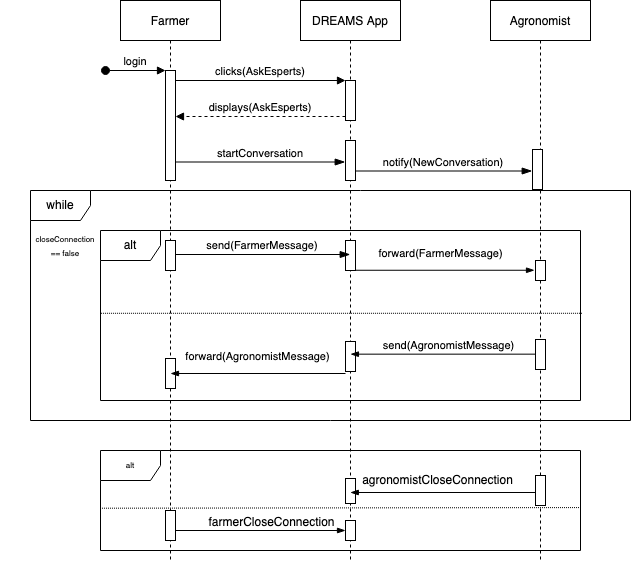
\includegraphics[scale=0.6]{Files/sequence_disgrams/thePNGs/farmer_askExperts.png}\\
\end{center}
text text hello describe
\begin{center}
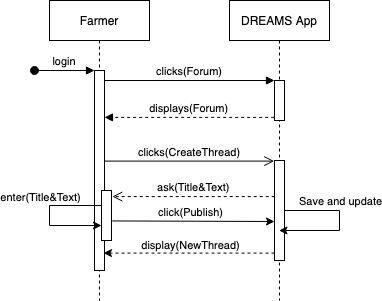
\includegraphics[scale=0.6]{Files/sequence_disgrams/thePNGs/farmer_createThread.png}\\
\end{center}
test test describe hello
\begin{center}
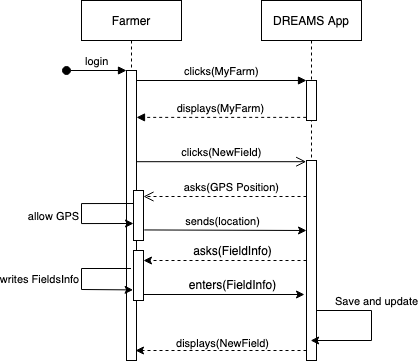
\includegraphics[scale=0.6]{Files/sequence_disgrams/thePNGs/farmer_newField.png}\\
\end{center}
hello hello why is there so much space 

\subsubsection{Agronomist}

\begin{center}
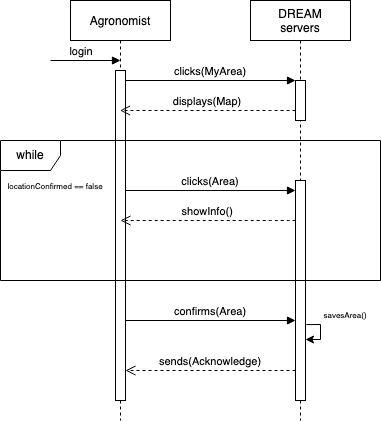
\includegraphics[scale=0.6]{Files/sequence_disgrams/thePNGs/agronomist_choosingLocation.png}\\
\end{center}


\begin{center}
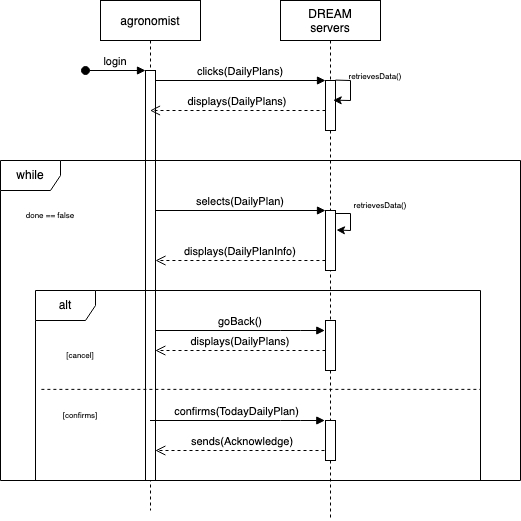
\includegraphics[scale=0.6]{Files/sequence_disgrams/thePNGs/agronomist_confirmPlan.png}\\
\end{center}

\begin{center}
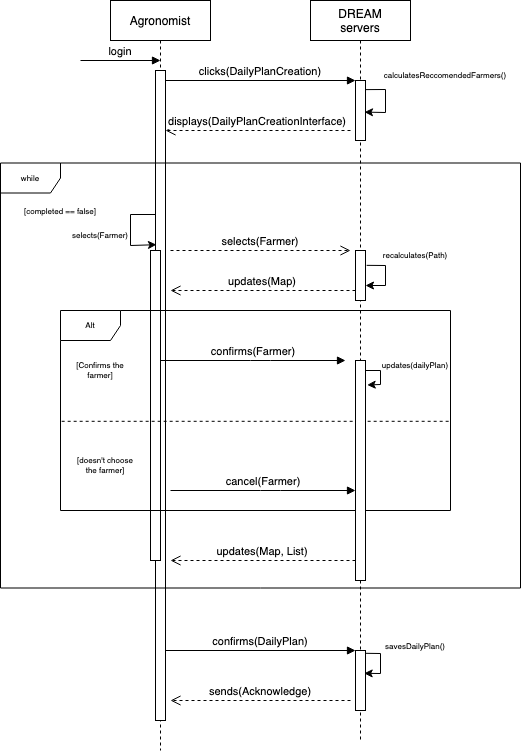
\includegraphics[scale=0.6]{Files/sequence_disgrams/thePNGs/agronomist_createPlan.png}\\
\end{center}

\begin{center}
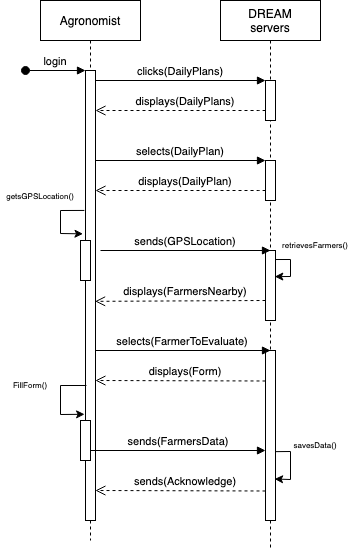
\includegraphics[scale=0.6]{Files/sequence_disgrams/thePNGs/agronomist_sendReport.png}\\
\end{center}

\subsubsection{Policy Maker}

\begin{center}
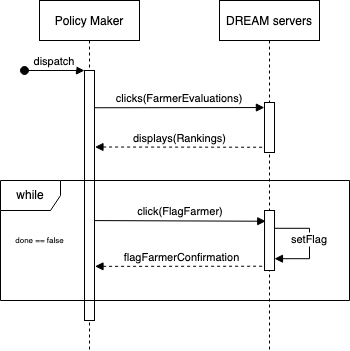
\includegraphics[scale=0.6]{Files/sequence_disgrams/thePNGs/policy_setFlag.png}\\
\end{center}

\begin{center}
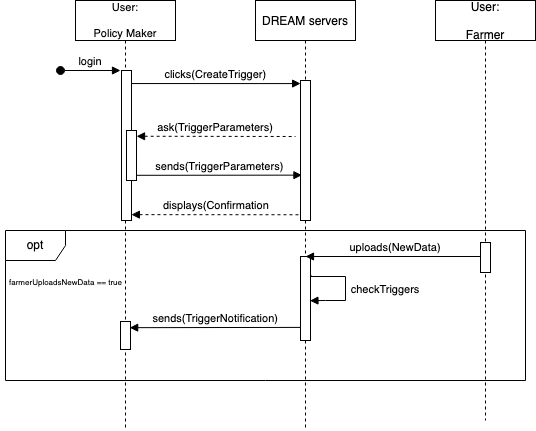
\includegraphics[scale=0.6]{Files/sequence_disgrams/thePNGs/policy_setTrigger.png}\\
\end{center}

\begin{center}
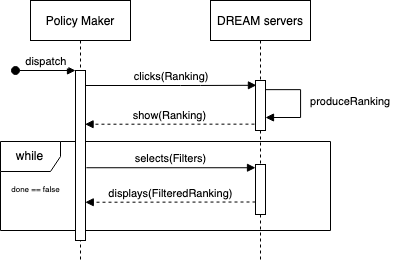
\includegraphics[scale=0.6]{Files/sequence_disgrams/thePNGs/policy_viewRanking.png}\\
\end{center}



%
%\textbf{EXAMPLE:} if the system determines that precipitation levels are decreasing and enabling a water scarcity crisis, policy makers should be able to see that identify that trend in the system and this can motivate them to enforce policy such as investing in water irrigation technologies that increase efficiency and reduce water waste. Once such policies are in place, telengana policy makers can identify if the new policy mediates the water scarcity problem. 
%\\

% \input{Files/usecases/usecase6.tex}
% .......


\subsection{Performance Requirements}
\subsection{Design Constraints}
\subsubsection{Standards compliance}
\subsubsection{Hardware limitations}
\subsubsection{Any other constraints}
\subsection{Software System Attributes}
\subsubsection{Reliability}
\subsubsection{Availability}
\subsubsection{Security}
\subsubsection{Maintainability}
\subsubsection{Portability}